

\tikzset{every picture/.style={line width=0.75pt}} %set default line width to 0.75pt        
\noindent
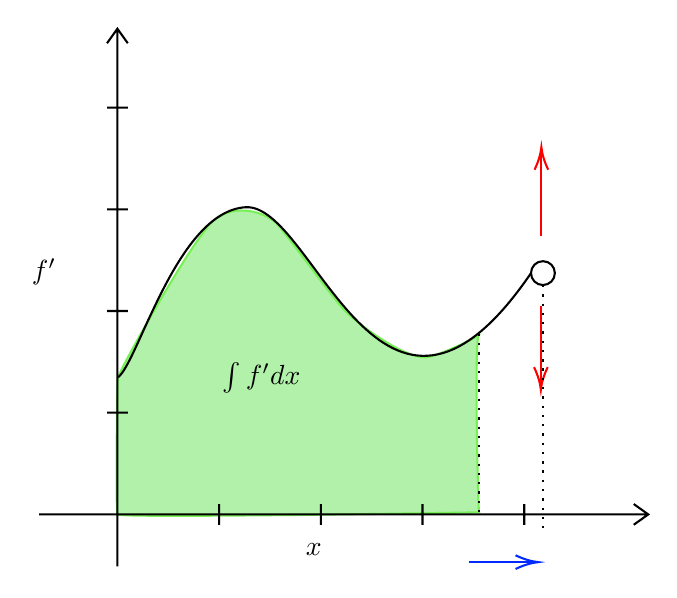
\begin{tikzpicture}[x=0.75pt,y=0.75pt,yscale=-1,xscale=1]
%uncomment if require: \path (0,300); %set diagram left start at 0, and has height of 300

%Shape: Polygon Curved [id:ds4987676772706314] 
\draw  [color={rgb, 255:red, 119; green, 240; blue, 85 }  ,draw opacity=1 ][fill={rgb, 255:red, 177; green, 241; blue, 169 }  ,fill opacity=1 ] (77,186) .. controls (77.5,183) and (113.5,118) .. (123.5,110) .. controls (133.5,102) and (148.5,106) .. (154.5,113) .. controls (160.5,120) and (180.21,147.41) .. (186.5,154) .. controls (192.79,160.59) and (217.5,179) .. (227.5,176) .. controls (237.5,173) and (253.5,165) .. (251,165) .. controls (248.5,165) and (250.5,251) .. (251,251) .. controls (251.5,251) and (77.5,254) .. (76.73,252) .. controls (75.96,250) and (76.5,189) .. (77,186) -- cycle ;
%Shape: Axis 2D [id:dp2444885928490862] 
\draw  (39,252) -- (332.5,252)(76.73,18) -- (76.73,277) (325.5,247) -- (332.5,252) -- (325.5,257) (71.73,25) -- (76.73,18) -- (81.73,25) (125.73,247) -- (125.73,257)(174.73,247) -- (174.73,257)(223.73,247) -- (223.73,257)(272.73,247) -- (272.73,257)(71.73,203) -- (81.73,203)(71.73,154) -- (81.73,154)(71.73,105) -- (81.73,105)(71.73,56) -- (81.73,56) ;
\draw   ;
%Shape: Circle [id:dp4961238584786192] 
\draw   (276,135.75) .. controls (276,132.57) and (278.57,130) .. (281.75,130) .. controls (284.93,130) and (287.5,132.57) .. (287.5,135.75) .. controls (287.5,138.93) and (284.93,141.5) .. (281.75,141.5) .. controls (278.57,141.5) and (276,138.93) .. (276,135.75) -- cycle ;
%Curve Lines [id:da30467668763713107] 
\draw    (77,186) .. controls (86.79,178.66) and (105.5,106) .. (138.5,104) .. controls (171.5,102) and (203.5,242) .. (276,135.75) ;
%Straight Lines [id:da36349385516051635] 
\draw [color={rgb, 255:red, 255; green, 0; blue, 0 }  ,draw opacity=1 ]   (281,118) -- (281,77) ;
\draw [shift={(281,75)}, rotate = 450] [color={rgb, 255:red, 255; green, 0; blue, 0 }  ,draw opacity=1 ][line width=0.75]    (10.93,-3.29) .. controls (6.95,-1.4) and (3.31,-0.3) .. (0,0) .. controls (3.31,0.3) and (6.95,1.4) .. (10.93,3.29)   ;
%Straight Lines [id:da23259457009514273] 
\draw [color={rgb, 255:red, 255; green, 0; blue, 0 }  ,draw opacity=1 ]   (280.75,151.5) -- (280.75,190) ;
\draw [shift={(280.75,192)}, rotate = 270] [color={rgb, 255:red, 255; green, 0; blue, 0 }  ,draw opacity=1 ][line width=0.75]    (10.93,-3.29) .. controls (6.95,-1.4) and (3.31,-0.3) .. (0,0) .. controls (3.31,0.3) and (6.95,1.4) .. (10.93,3.29)   ;
%Straight Lines [id:da3927869746462661] 
\draw  [dash pattern={on 0.84pt off 2.51pt}]  (281.75,141.5) -- (281.75,260) ;
%Straight Lines [id:da5865427634124499] 
\draw [color={rgb, 255:red, 0; green, 42; blue, 255 }  ,draw opacity=1 ]   (246,275) -- (277.5,275) ;
\draw [shift={(279.5,275)}, rotate = 180] [color={rgb, 255:red, 0; green, 42; blue, 255 }  ,draw opacity=1 ][line width=0.75]    (10.93,-3.29) .. controls (6.95,-1.4) and (3.31,-0.3) .. (0,0) .. controls (3.31,0.3) and (6.95,1.4) .. (10.93,3.29)   ;
%Straight Lines [id:da8199987268344746] 
\draw  [dash pattern={on 0.84pt off 2.51pt}]  (251,165) -- (251,251) ;

% Text Node
\draw (34,127.4) node [anchor=north west][inner sep=0.75pt]    {$f'$};
% Text Node
\draw (166,264.4) node [anchor=north west][inner sep=0.75pt]    {$x$};
% Text Node
\draw (126,177.4) node [anchor=north west][inner sep=0.75pt]    {$\int f'dx$};


\end{tikzpicture}
